\documentclass[../EDF Master Thesis.tex]{subfiles}

\begin{document}
\ac{freertos} ist ein Echtzeitbetriebssystem für eingebettete Systeme, welches unter der freizügigen Open-Source Lizenz \href{https://de.wikipedia.org/wiki/MIT-Lizenz}{MIT} steht.
Außerdem ist der Scheduler des Betriebsystems zwischen präemptiver und kooperativer Betrieb konfigurierbar um verschiedene Einsatzzwecke abzudecken \parencite{wiki:002}.
\ac{freertos} unterstützt über 40 Mikrocontroller-Architekturen, um eine größere Bandbreite zu erreichen \parencite{freertos}.
Für nicht unterstütze Architekturen stellt \ac{freertos} eine Portierungs-Anleitung zur Verfügung, welche als Unterstützung bei der Portierung von \ac{freertos} auf andere \ac{cpu}s dient \autocite{freertos_port}.
\ac{freertos} ist einfach zu implementieren und der Kernel unterstützt Multithreading, Warteschlangen, Semaphore, Software-Timer, Mutexes und Eventgruppen \parencite{freertos-features}.
Des Weiteren stellt \ac{freertos} unter der Bezeichnung "FreeRTOS Plus" verschiedene Erweiterungen zur Verfügung, welche erweiterte Funktionen bereitstellen \parencite{freertos-extensions}.
Folgende Erweiterungen sind zum Stand dieser Arbeit verfügbar:
\begin{itemize}
    \item \textbf{FreeRTOS + TCP}: Socketbasiertes \ac{tcp}/\\\ac{udp}/\ac{ip} Interface.
    \item \textbf{Application Protocols}: \ac{mqtt} und \\\ac{http} Anwendungsprotokolle für \ac{iot}.
    \item \textbf{coreJson}: Effizienter Parser für \ac{json}
    \item \textbf{corePKCS\#11}: Verschlüsselungs \ac{api}-Layer
    \item \textbf{FreeRTOS + IO}: Erweiterung für Peripheriegeräte
    \item \textbf{FreeRTOS + CLI}: Effiziente \ac{cli}-Eingaben
\end{itemize}
\begin{center}
    (\ac{iaa} \cite{freertos-extensions})
\end{center}

Im Zuge dieser Masterarbeit wurde als einziges der Stack '\ac{freertos} + \acs{tcp}' für die Verbindung zwischen Computer und Mikrocontroller verwendet.
Wobei die Integration von anderen Erweiterungen keinen Einfluss auf den in dieser Arbeit implementierten \ac{edf}-Scheduler hat.

\subsubsection{\ac{freertos} Scheduling Richtlinie} \label{section:freertos_scheduling_richtlinie}
Der \ac{freertos}-Scheduler arbeitet prioritätsbasiert und beinhaltet standardmäßig zwei Eigenschaften:
\begin{itemize}
    \item \textbf{Time Slicing Scheduling Policy}: Tasks mit gleicher Priorität erhalten die gleiche Anteile an \ac{cpu}-Zeit, dieses Verfahren ist auch als 'Round-Robin Algorithmus' bekannt.
    \item \textbf{Fixed Priority Preemptive Scheduling}: Es wird immer die Task  mit der höchsten Priorität ausgeführt.
                                                         Das bedeutet eine niedriger priorisierte Task bekommt nur \ac{cpu}-Zeit, wenn die höher priorisierten Tasks nicht den 'ready'-Status besitzen.
                                                         Teilen sich zwei Tasks gleichzeitig die höchste Priorität, tritt die Time Slicing Scheduling Policy in Kraft.
\end{itemize}
Um einen oder beide dieser Eigenschaften abzuschalten, kann dies unter der Datei \\'FreeRTOSConfig.h', wie in \autoref{code:freertos_scheduling_policies} dargestellt, abgeändert werden.
Je nach gewünschter Anwendung könnten diese Optionen diese negativ oder positiv beeinflussen \parencite{freertos-scheduling-policy}.
\begin{lstlisting}[language=C, caption=FreeRTOS Scheduling Policy Properties, label=code:freertos_scheduling_policies]
    #define configUSE_PREEMPTION                    ( 1 )
    #define configUSE_TIME_SLICING                  ( 1 )
\end{lstlisting}


\subsubsection{Overhead und Footprint} \label{section:overhead_und_footprint}
Die Dauer eines Context Switches, auch Taskwechsel genannt, zwischen zwei Tasks ist abhängig von der Portierung, dem Compiler und der Konfiguration von FreeRTOS.
FreeRTOS selbst gibt ein Beispiel anhand einer Cortex-M3 CPU eine Taskwechsel Zeit von 84 \ac{cpu} Zyklen an \parencite{freertos-overhead}.
Typischerweise besitzt ein \ac{freertos} Kernel Binary Image eine Größe zwischen 6Byte und 12kByte \parencite{freertos-footprint}.

\clearpage

\subsubsection{Task States} \label{section:task_states}
In FreeRTOS erzeugte Tasks können vier verschiedene Zustände erreichen.
Diese Zustände ermöglichen komplexere Algorithmen zu implementieren und sehen wie folgt aus:

\begin{itemize}
    \item \textbf{Running}: Die Task wird gerade ausgeführt.
    \item \textbf{Ready}: Die Task ist bereit zur Ausführung.
    \item \textbf{Blocked}: Die Task wartet auf ein Event, kann nicht ausgeführt werden.
    \item \textbf{Suspended}: Die Task wurde von der Anwendung deaktiviert.
\end{itemize}
\begin{center}
    \parencite{freertos-task-states}
\end{center}

Ein Ablaufdiagramm der einzelnen Zustände und deren Wechsel mit Hilfe von \ac{freertos}-Funktionen wird in \autoref{fig:FreeRTOS_Task_States} dargestellt.
Dabei wird erläutert, mit welchen \ac{freertos}-Funktionen oder Events den Statuswechsel auslösen \autocite{freertos-task-states}.

\begin{figure}[H]
    \centering
    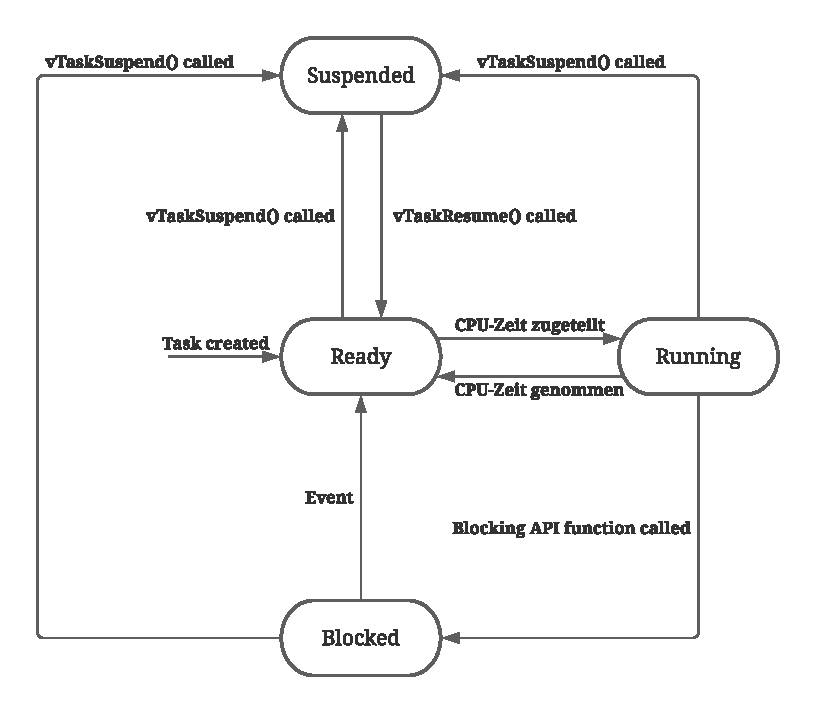
\includegraphics[height=10cm, width=10cm]{./attachments/FreeRTOS_Task_States.pdf}
    \caption[FreeRTOS Task States]{FreeRTOS Task States (\ac{iaa} \cite{freertos-task-states})}
    \label{fig:FreeRTOS_Task_States}
\end{figure}

\subsubsection{Idle Task} \label{section:idle_task}
Die \ac{freertos} Idle Task wird immer dann aufgerufen, wenn keine Task ausgeführt werden kann.
Dabei wird die \ac{freertos} Idle Task automatisch beim Start des \ac{freertos}-Schedulers mit der niedrigsten verfügbaren Priorität erstellt, um keine Tasks im 'ready' Status zu blockieren.
Das heißt die Idle Task wird nur ausgeführt, wenn es keine Task mit einer höheren Priorität gibt, oder keine Task mit einer höheren Priorität sich im 'ready' Status befindet.
Sollte eine Task die gleiche Priorität mit der Idle Task teilen, wird die \ac{cpu}-Zeit, bei Standardkonfiguration, zwischen den zwei Tasks aufgeteilt.
Des Weiteren wird die Idle Task in \ac{freertos} Standardkonfiguration mit der Priorität 0, also der niedrigsten Priorität gestartet.
Beim Ausführen der \ac{freertos} Idle Task wird nicht mehr benötigter zugewiesener Speicher gelöscht und sollte somit regelmäßig \ac{cpu}-Zeit bekommen, da im schlimmsten Fall der Arbeitsspeicher überlaufen kann.
Des Weiteren kann mit der Flag, wie in \autoref{code:freertos_idle_task_hook_flag} zu sehen, der Idle Task Hook aktiviert werden.
Der Idle Task Hook wird bei jedem Aufruf der Idle Task ausgeführt und ermöglicht dem Benutzer dabei einen zusätzlichen Code auszuführen.
Dies kann für verschiedene Einsatzbereiche benutzt werden, wie beispielsweise um den Mikrocontroller in den Energiesparmodus zu setzen \autocite{freertos_idle_task}.

\begin{lstlisting}[language=C, caption=FreeRTOS Idle Task Hook Flag, label=code:freertos_idle_task_hook_flag]
    #define configUSE_IDLE_HOOK                     ( 1 )
\end{lstlisting}


\subsubsection{Interrupts} \label{section:interrupts}
Interrupts werden durch ein Ereignis ausgelöst, wie z.B. einem bestimmten Wert eines Timers ausgelöst und führen zur einer Unterbrechung der aktuellen Programmausführung, um in der Regel kurzen, aber zeitlich kritischen, Vorgang abzuarbeiten.
Nach der Unterbrechungsanforderung (\ac{irq}) führt der Prozessor eine Unterbrechungsroutine (\ac{isr}) mit erweiterten Privilegien aus.
Im Anschluss wird der vorherige Zustand des Prozessors wiederhergestellt und die vorherige Ausführung an der unterbrochenen Stelle fortgesetzt \parencite{grundkurs_betriebssysteme, wiki:008}.


\subsubsection{\ac{freertos} SysTick} \label{section:freertos_sys_tick}
Der \ac{freertos} SysTick, auch System Tick genannt, ist fundemental für die Taskwechsel in \ac{freertos}.
Dieser Interrupt wird standardmäßig jede Millisekunde aufgerufen.
Dabei bietet der Wert eine gute Balance zwischen Taskgeschwindigkeit und Overhead von Taskwechsel.
Bei jedem SysTick wird die \ac{freertos} Funktion 'vTaskSwitchContext()' aufgerufen.
Die Funktion selbst überprüft ob eine höher priorisierte Task unblocked, also ausführbar (ready) geworden ist und falls dies zutrifft wird ein Taskwechsel auf die höher priorisierte Task durchgeführt \autocite{freertos_systick}.

\subsubsection{\ac{freertos} Queues} \label{section:queues}
Queues, zu Deutsch Warteschlangen, werden oft auch außerhalb von \ac{freertos} für die sichere Kommunikation zwischen verschiedenen Tasks und/oder Interrupts verwendet.
Bei Queues wird oft das Prinzip \ac{fifo} verwendet, bei dem die Daten, welche zu erst in die Queue gesendet wurden, als erstes weiterverarbeitet werden.
\end{document}
